\begin{figure}[ht]
\begin{nexample}
  We will show that the Petersen graph is non-planar. Here are a
  few strategies we can use to do so. Let us also denote the
  Petersen graph as \(G\).
  \begin{enumerate}
    \item Use the number of edge inequality. Indeed, we can see
      that there are 15 edges in this graph. However, \(3n-6 =
      24\). So, this test is still inconclusive.

    \item We can try to identity a \(K_{3, 3}\) subdivision of
      \(G\). 
      \begin{center}
        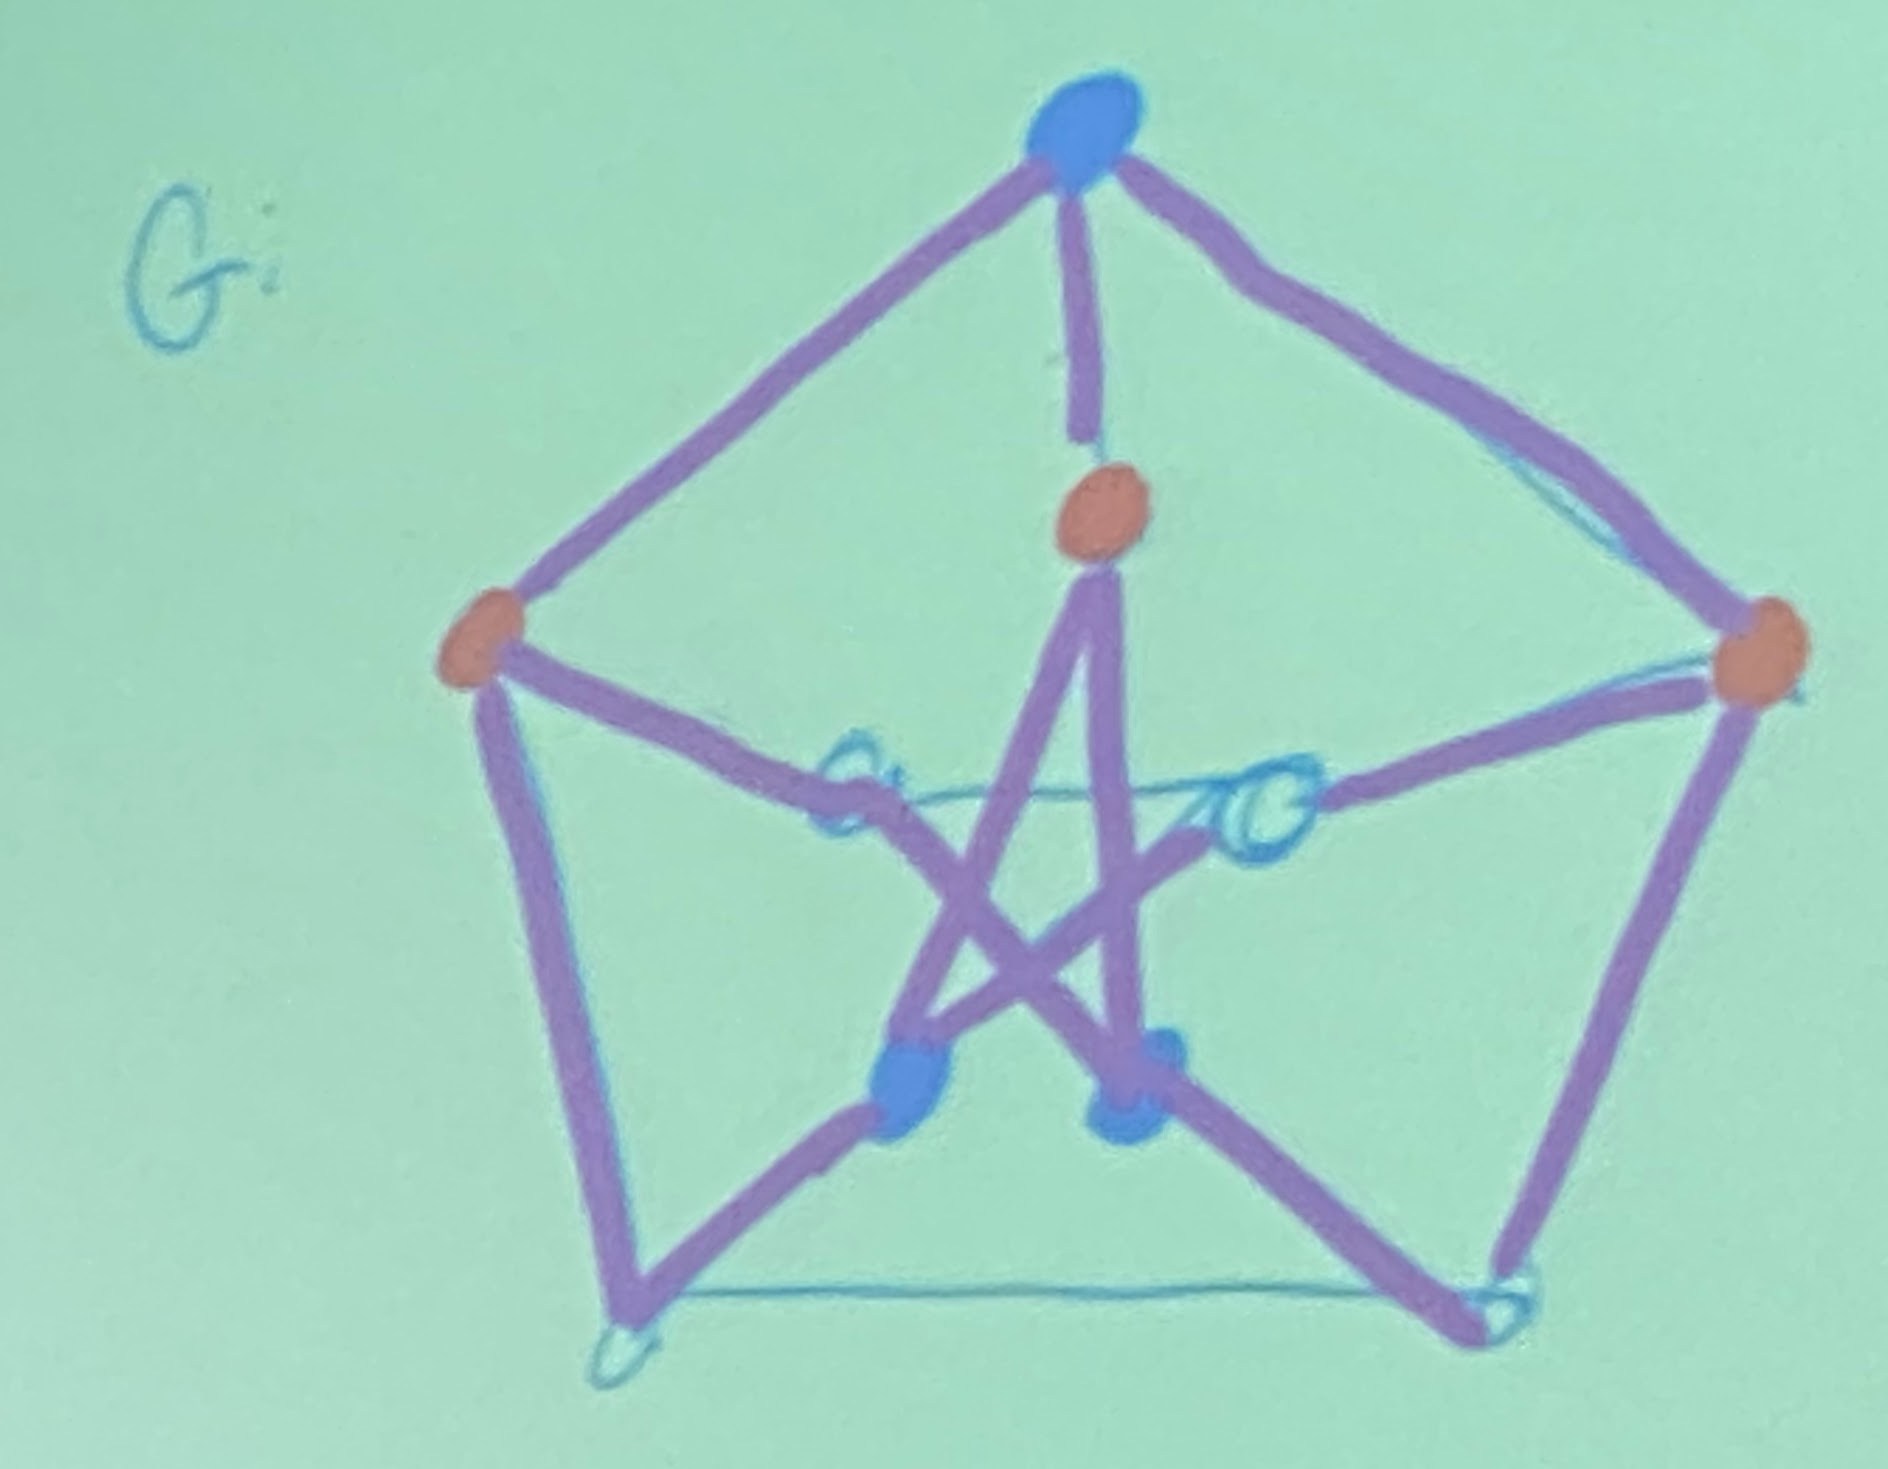
\includegraphics[width=0.3\textwidth]{figures/l14/petersen-k33}
      \end{center}
  \end{enumerate}
\end{nexample}
\end{figure}

\begin{distraction}
  Kuratowski's Theorem (1930) is older than Wagner's Theorem
  (1937). In fact, Wagner deduced his theorem using Kuratowski's
  Theorem. However, people nowadays can prove Wagner's Theorem by
  itself without using Kuratowski's Theorem and this \textit{more
  modern} proof is simpler than one with Kuratowski's Theorem.
\end{distraction}

\chapter{Coloring}

\section{Core Definitions}

\begin{definition}[\(k\)-colorable]
  A graph \(G\) is \textit{\(k\)-colorable} if we can assign 
  colors \(c_1, c_2, \ldots, c_k\) to the vertices of \(G\) such
  that no two adjacent vertices has the same color.
\end{definition}

\begin{definition}[Chromatic Number]
  The \textit{chromatic number} of a graph \(G\), denoted
  \(\chi(G)\), is the smallest number \(k\) such that \(G\) is
  \(k\)-colorable.
\end{definition}

\begin{nexample}
  Let us determine the chromatic numbers of trees, bipartite
  graphs, \(C_n\), \(W_n\), \(K_n\), and the Petersen graph.
  \begin{itemize}
    \item A tree \(T\) has no cycle so \(\chi(T) = 2\) 
    \item Similarly, any bipartite graph \(G\) do not have edges
      between its own partite so \(\chi(G) = 2\) as well
    \item For cyclic graphs \(C_n\), we need to separate by
      cases:
      \begin{enumerate}[label=\Roman*.]
        \item If \(n=1\), then \(\chi(C_n)=1\)
        \item If \(n\) even, then \(\chi(C_n) = 2\)
        \item If \(n\) odd, then \(\chi(C_n) = 3\)
      \end{enumerate}
    \item Similar to cyclic graphs, the chromatic numbers of 
      \(W_n\)'s will be separated by cases as well:
      \begin{enumerate}[label=\Roman*.]
        \item If \(n\) even, then \(\chi(W_n) = 3\); 2 for the
          outside and one for the middle
        \item If \(n\) odd, then \(\chi(W_n) = 4\); 3 for the
          outside and one for the middle
      \end{enumerate}
    \item For \(K_n\)'s, \(\chi(K_n) = n\) since every vertex is
      adjacent to the rest of the vertices
    \item For the Petersen Graph, its chromatic number is 3
  \end{itemize}
\end{nexample}
